\documentclass[11pt,a4paper]{article}

% --- Packages ---
\usepackage[utf8]{inputenc}
\usepackage[T1]{fontenc}
\usepackage{geometry}
\geometry{margin=1in, headheight=14pt}
\usepackage{lmodern}
\usepackage{graphicx}
\usepackage{xcolor}
\usepackage{listings}
\usepackage{hyperref}
\usepackage{caption}
\usepackage{booktabs}
\usepackage{float}
\usepackage{fancyhdr}
\usepackage{titlesec}
\usepackage[most]{tcolorbox}
\usepackage{tikz}
\tcbuselibrary{listings}
%\usepackage{microtype}

% --- Defined Colors ---
\definecolor{codegray}{rgb}{0.5,0.5,0.5}
\definecolor{codepurple}{rgb}{0.58,0,0.82}
\definecolor{backcolour}{rgb}{0.95,0.95,0.96}
\definecolor{codeblue}{rgb}{0.0,0.2,0.6}
\definecolor{codegreen}{rgb}{0.0,0.5,0.0}
\definecolor{darkgray}{rgb}{0.2,0.2,0.2}

% --- tcolorbox styling (mintedbox-like) ---
\newtcblisting{mintedbox}[2][]{
    arc=3pt,
    boxrule=0.5pt,
    colback=backcolour,
    colframe=codeblue!60,
    listing only,
    breakable,
    enhanced,
    listing options={
        language=#2,
        basicstyle=\ttfamily\small\color{darkgray},
        keywordstyle=\color{codeblue}\bfseries,
        commentstyle=\color{codegray}\itshape,
        stringstyle=\color{codegreen},
        numbers=left,
        numberstyle=\tiny\color{codegray},
        stepnumber=1,
        numbersep=10pt,
        showstringspaces=false,
        breaklines=true,
        tabsize=4,
    },
    title=\texttt{#2},
    coltitle=white,
    colbacktitle=codeblue!80,
    fonttitle=\bfseries\ttfamily\small,
    left=15pt,
    borderline west={2pt}{0pt}{codeblue},
    attach boxed title to top right={yshift=-2mm, xshift=-5mm},
    boxed title style={sharp corners=all, rounded corners=southwest, boxrule=0.5pt, colframe=codeblue!80},
    #1
}

% --- tcbinputlisting for Appendix (mintedbox style) ---
\newtcbinputlisting{\codeblock}[2]{
    arc=3pt,
    boxrule=0.5pt,
    colback=backcolour,
    colframe=codeblue!60,
    listing only,
    breakable,
    enhanced,
    listing options={
        language=Python,
        basicstyle=\ttfamily\small\color{darkgray},
        keywordstyle=\color{codeblue}\bfseries,
        commentstyle=\color{codegray}\itshape,
        stringstyle=\color{codegreen},
        numbers=left,
        numberstyle=\tiny\color{codegray},
        stepnumber=1,
        numbersep=10pt,
        showstringspaces=false,
        breaklines=true,
        tabsize=4,
    },
    listing file={#1},
    title=\texttt{#2},
    coltitle=white,
    colbacktitle=codeblue!80,
    fonttitle=\bfseries\ttfamily\small,
    left=15pt,
    borderline west={2pt}{0pt}{codeblue},
    attach boxed title to top right={yshift=-2mm, xshift=-5mm},
    boxed title style={sharp corners=all, rounded corners=southwest, boxrule=0.5pt, colframe=codeblue!80}
}

% --- Hyperref Setup (Blue Links) ---
\hypersetup{
    colorlinks=true,
    linkcolor=blue,
    filecolor=blue,      
    urlcolor=blue,
    pdftitle={MIMIC-IV Forecasting Report},
}

% --- Header & Footer (Initialized after front matter) ---
\fancyhf{}
\fancyfoot[C]{\thepage}
\renewcommand{\headrulewidth}{0pt}

\begin{document}
\thispagestyle{empty}
\begin{tikzpicture}[remember picture, overlay]
    % Sidebar
    \fill[codeblue!10] (current page.north west) rectangle ([xshift=6cm]current page.south west);
    \fill[codeblue!80] (current page.north west) rectangle ([xshift=0.5cm]current page.south west);
    
    % Decorative Pattern in Sidebar
    \foreach \i in {1,...,20} {
        \draw[codeblue!30, line width=0.5pt] ([xshift=1cm, yshift=-\i*1cm]current page.north west) -- ([xshift=5.5cm, yshift=-\i*1cm-2cm]current page.north west);
    }
    
    % Title Block (Anchored to Right)
    \node[anchor=north east, align=right, text width=12cm] at ([xshift=-1.5cm, yshift=-8cm]current page.north east) {
        {\fontsize{38}{48}\selectfont \textbf{Time-Series Modelling and}}\\ 
        \vspace{0.4cm}
        {\fontsize{42}{52}\selectfont \textbf{Forecasting}}\\
        \vspace{2cm}
        {\Large \textit{Using the MIMIC-IV Clinical Database}}\\
        \vspace{4cm}
        \rule{8cm}{2pt}\\
        \vspace{1.5cm}
        {\Huge \textbf{Irine Maria Jose}}\\
        \vspace{6cm}
        {\color{gray} \Large \today}\\
        \vspace{1cm}
        \textbf{\Large Technical Research Report}
    };
\end{tikzpicture}
\vfill\null
\clearpage

\pagenumbering{roman}
\tableofcontents
\clearpage
\pagestyle{fancy}
\pagenumbering{arabic}

\section{Introduction and Objective}
This report details the end-to-end development of a hemodynamic forecasting pipeline using the MIMIC-IV Clinical Database (Demo v2.2). The primary objective is to predict \textbf{Mean Arterial Pressure (MAP)} at a 6-hour forecast horizon using clinical history, including vital signs, labs, and interventions.

\section{Dataset Engineering}
\subsection{Data Source and Extraction}
The MIMIC-IV demo dataset was utilized, targeting adult patients with an ICU stay of at least 6 hours. High-resolution vital signs (Mean Arterial Pressure, Heart Rate, SpO2) and sparse laboratory measurements (Creatinine, Lactate, WBC) were extracted and temporalized.

\begin{mintedbox}[title=Data Extraction Logic]{Python}
def load_chart_vitals(cohort):
    # Filter chartevents for specific Item_IDs (MAP, HR, SpO2, etc.)
    ce = pd.read_csv('chartevents.csv', usecols=['stay_id', 'charttime', 'itemid', 'valuenum'])
    ce = ce[(ce['itemid'].isin(ALL_CHART_IDS)) & (ce['stay_id'].isin(stay_ids))].copy()
    
    # Standardization & Physiological Filtering
    bounds = {'MAP': (20, 200), 'HR': (20, 300), 'Temperature': (25, 45)}
    for var, (lo, hi) in bounds.items():
        mask = (ce['variable'] == var) & (ce['valuenum'] >= lo) & (ce['valuenum'] <= hi)
        parts.append(ce[mask])
    return pd.concat(parts)
\end{mintedbox}

\subsection{Alignment and Tiered Imputation}
Raw EHR data is inherently asynchronous. All variables were aligned on a 1-hour grid relative to ICU admission. Given the high missingness in labs ($>90\%$), a tiered imputation strategy was implemented: forward-fill with variable caps followed by linear interpolation. This method was selected to preserve physiological fidelity better than simple mean-fill, ensuring that temporal gradients in vital signs are maintained.

\begin{mintedbox}[title=Tiered Imputation Strategy]{Python}
# Tier 1: forward-fill (4h vitals, 24h labs)
for col in vital_cols:
    df[col] = df.groupby('stay_id')[col].transform(lambda s: s.ffill(limit=4).bfill(limit=2))
for col in lab_cols:
    df[col] = df.groupby('stay_id')[col].transform(lambda s: s.ffill(limit=24).bfill(limit=12))

# Tier 2: Linear interpolation for gradient preservation
for col in ALL_VALUE_COLS:
    df[col] = df.groupby('stay_id')[col].transform(lambda s: s.interpolate(method='linear', limit=6))
\end{mintedbox}

\section{Quality Control and EDA}
\subsection{Cohort Selection and Attrition}
The filtering process ensures physiological reliability. Patients with extreme sensor artifacts or insufficient records were excluded.

\begin{figure}[H]
    \centering
    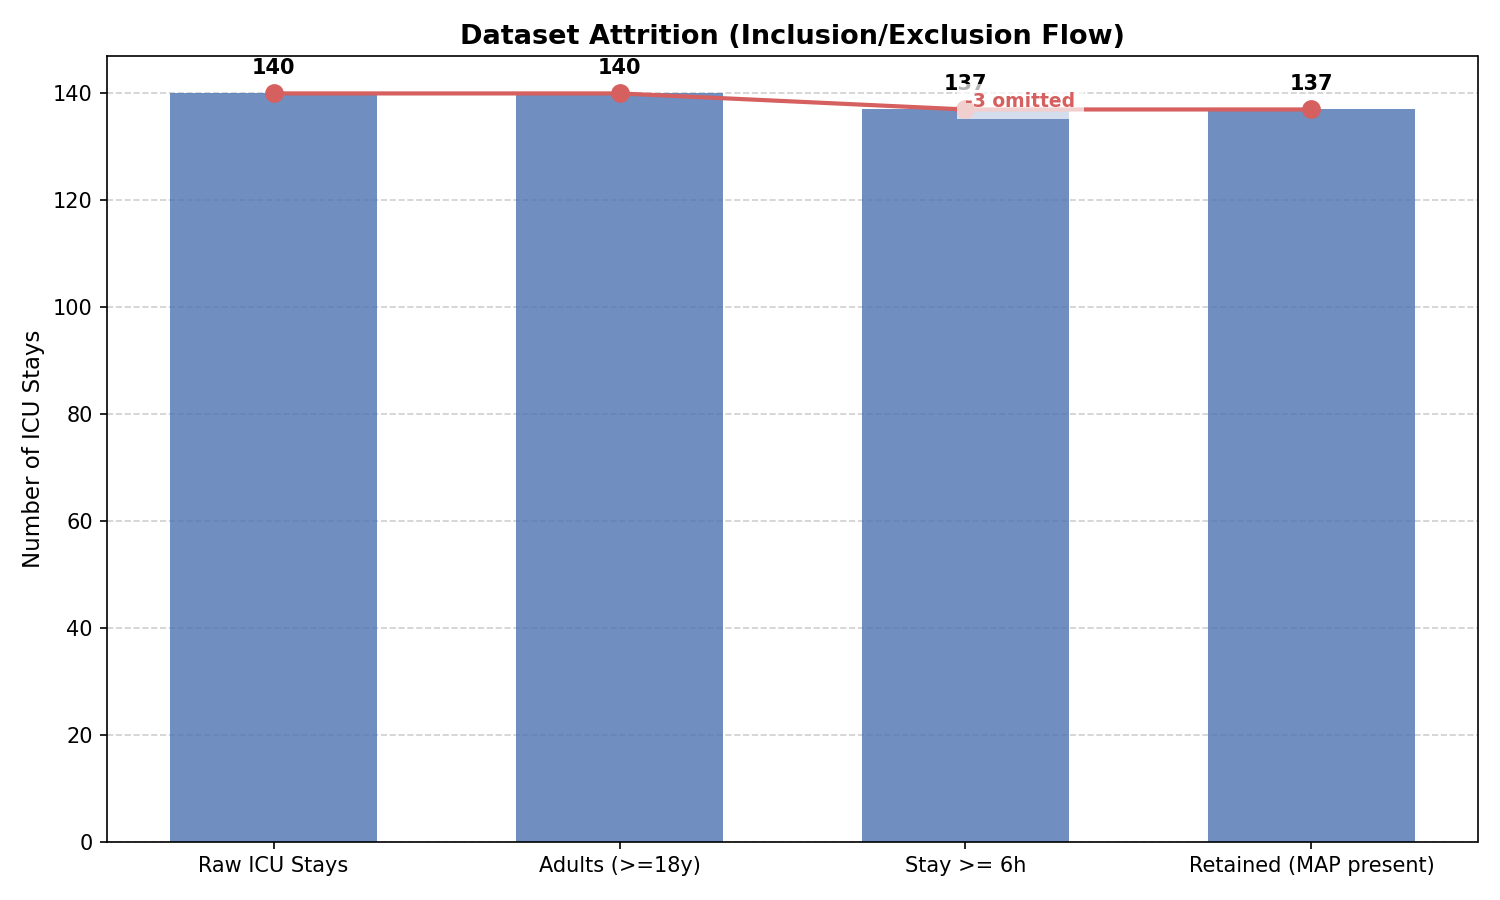
\includegraphics[width=0.8\textwidth]{outputs/qc/dataset_attrition.png}
    \caption{Dataset Attrition Flowchart}
\end{figure}

\subsection{Sampling Density and Missingness}
Vital signs exhibit high sampling density, whereas lab values remain sparse. MAP was selected as the target due to its continuous representation, vital for high-accuracy forecasting.

\begin{figure}[H]
    \centering
    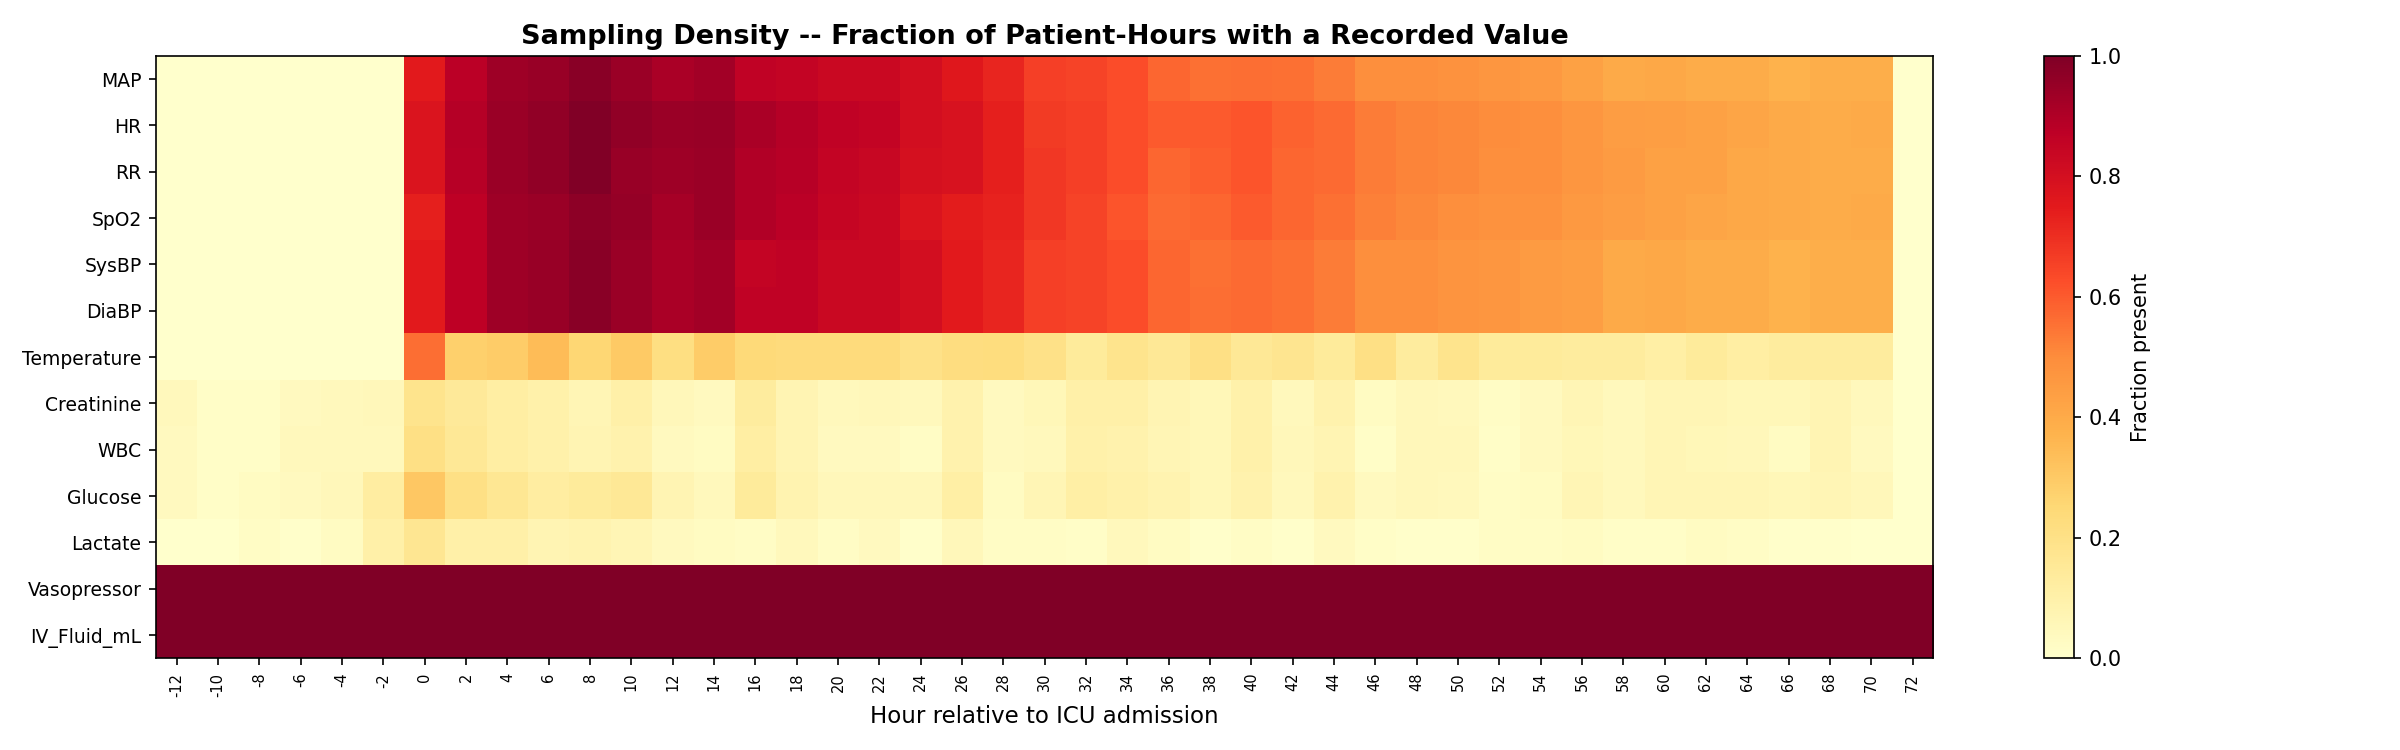
\includegraphics[width=1.0\textwidth]{outputs/qc/sampling_density_heatmap.png}
    \caption{Hourly Sampling Density (Fraction Present)}
\end{figure}

\begin{figure}[H]
    \centering
    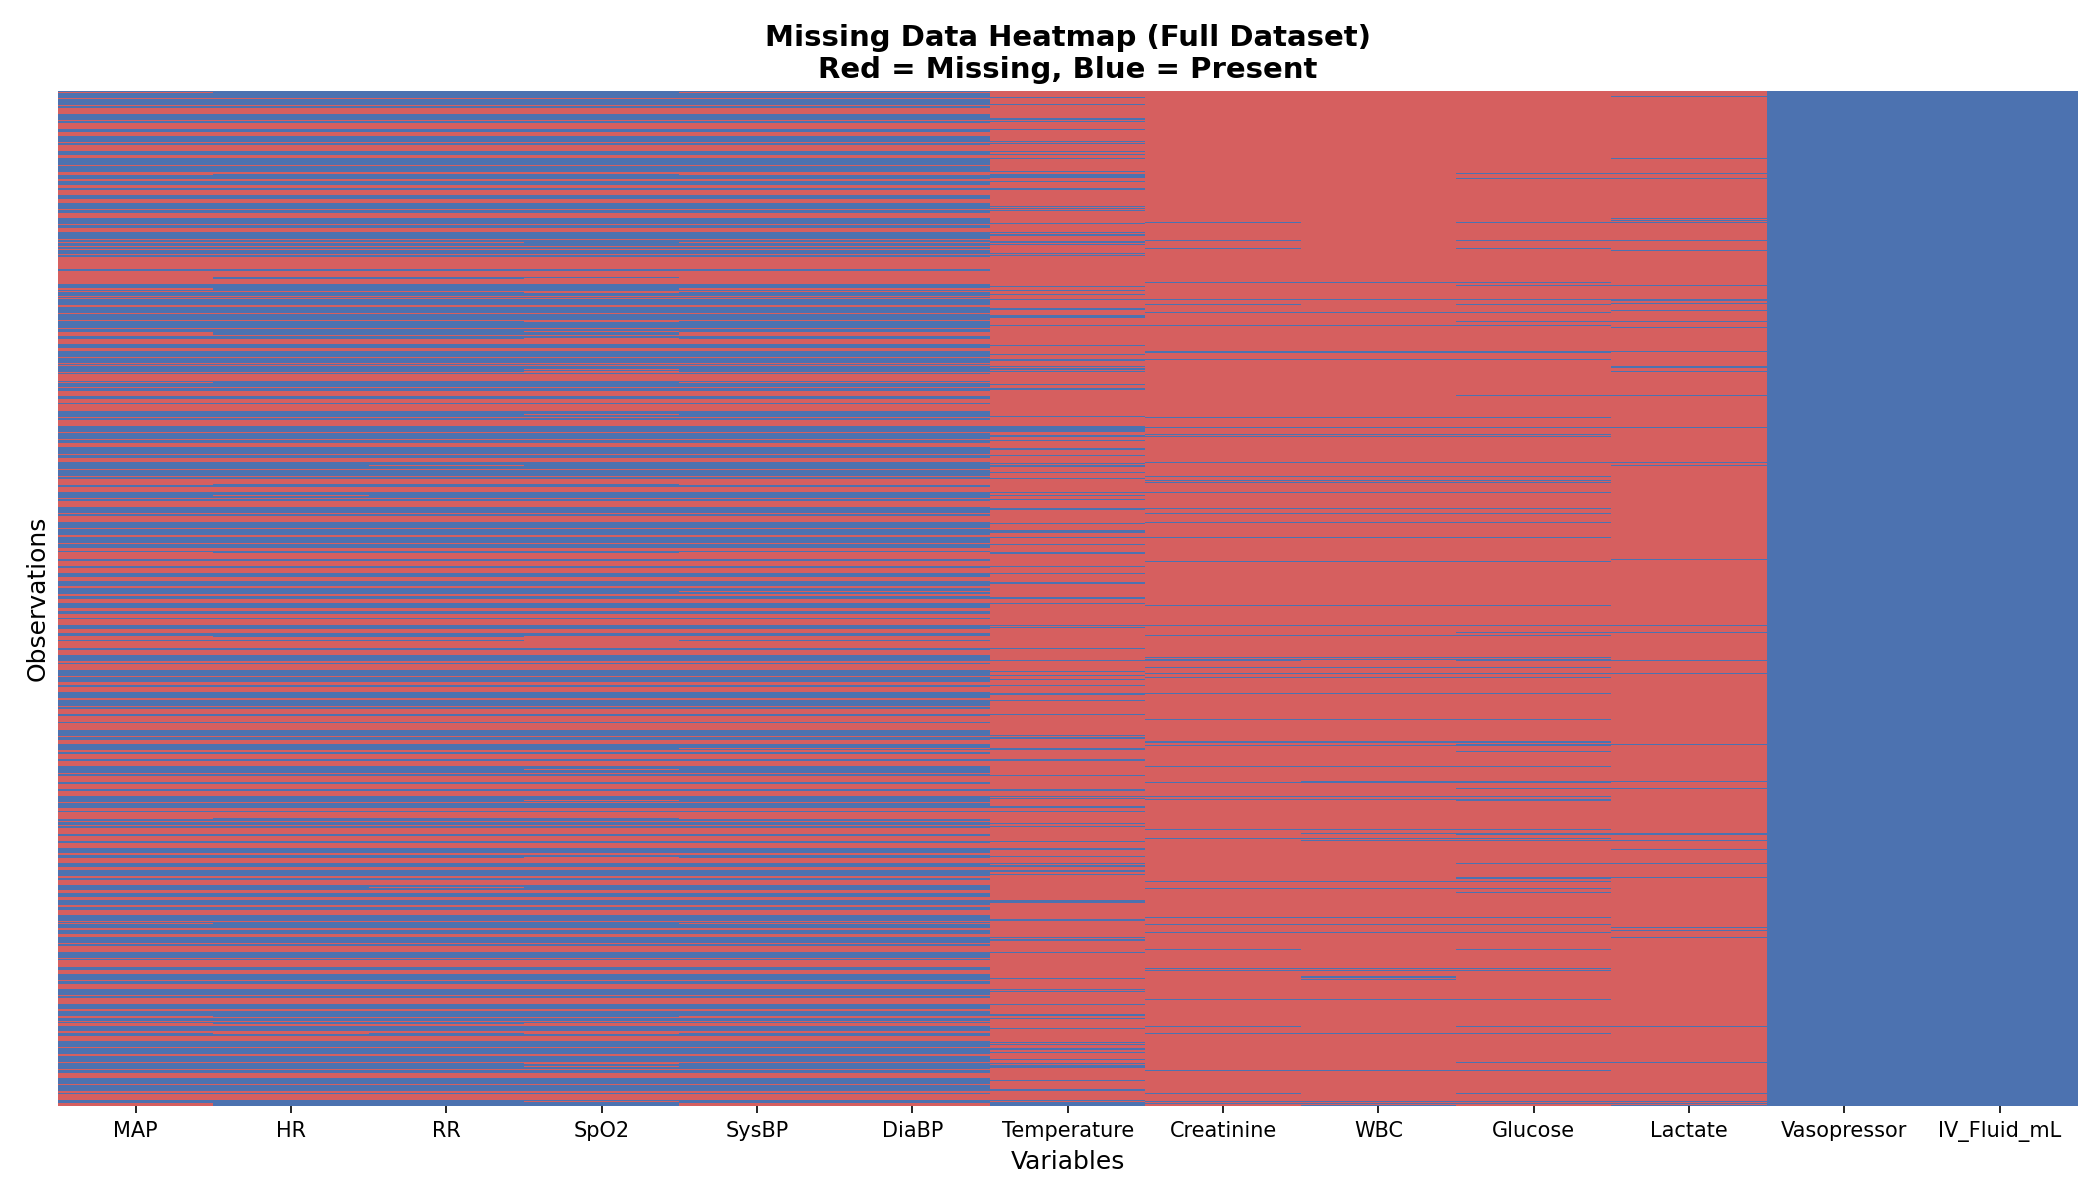
\includegraphics[width=1.0\textwidth]{outputs/eda/missing_data_heatmap.png}
    \caption{Temporal Missingness Heatmap (Raw Data)}
\end{figure}

\begin{figure}[H]
    \centering
    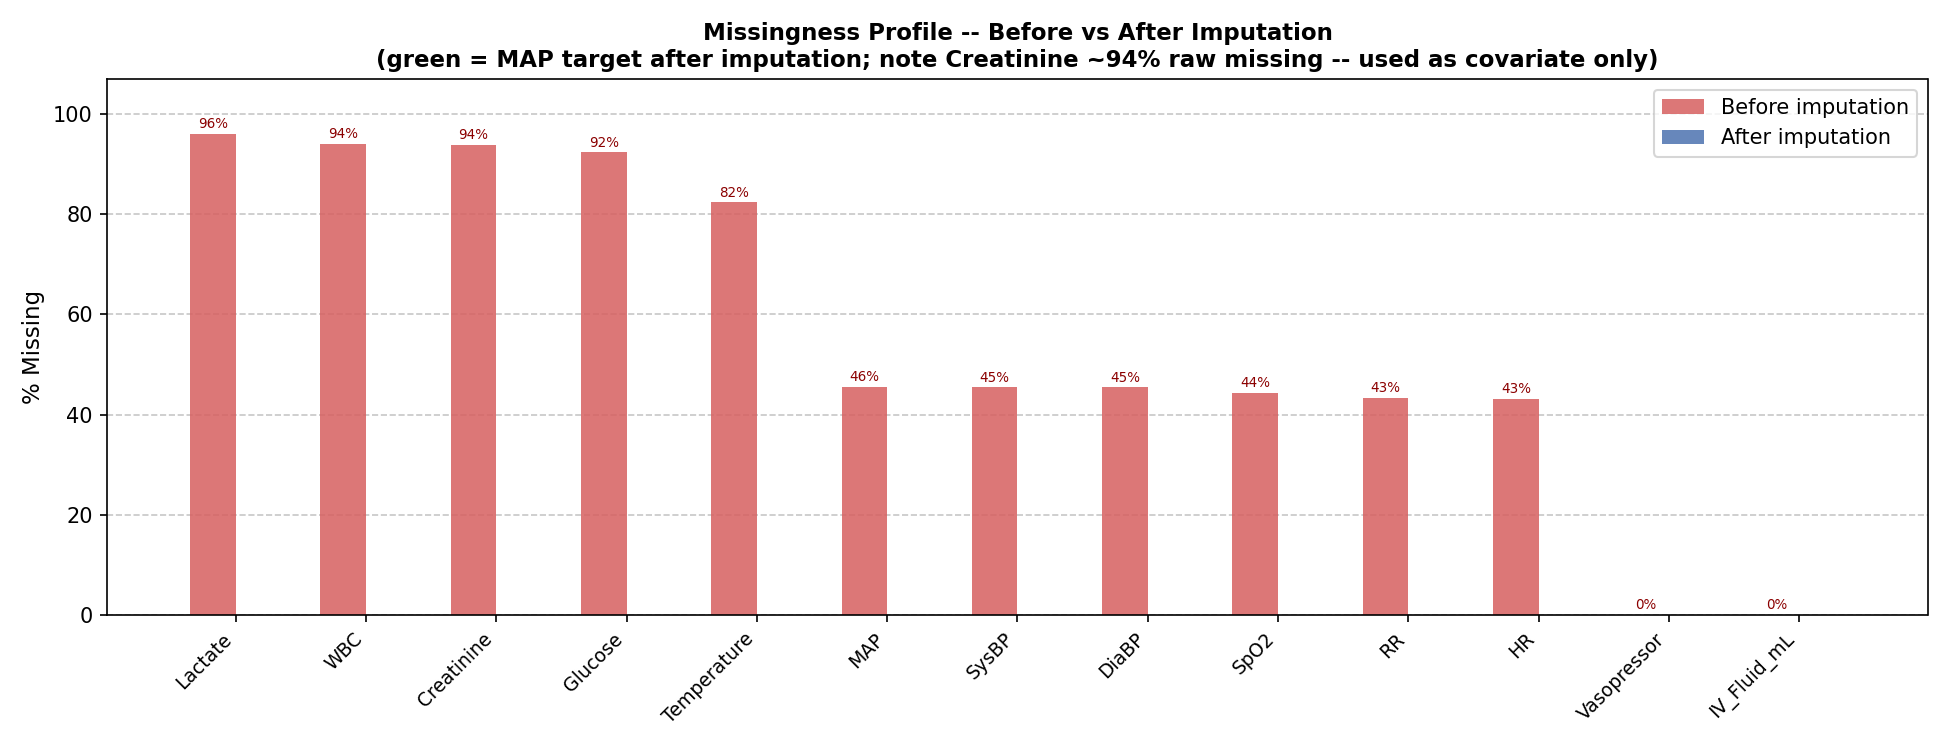
\includegraphics[width=0.8\textwidth]{outputs/qc/missingness_profile.png}
    \caption{Missingness Profile: Before vs After Imputation}
\end{figure}

\subsection{Split Consistency and Patient Trajectories}
To ensure the integrity of the predictive modeling, the distribution of the target variable (MAP) was validated across train, validation, and test splits. Figure \ref{fig:map_dist} confirms distributional consistency, mitigating the risk of split bias. Furthermore, individual patient trajectories were examined to understand physiological variability (Figure \ref{fig:trajectories}).

\begin{figure}[H]
    \centering
    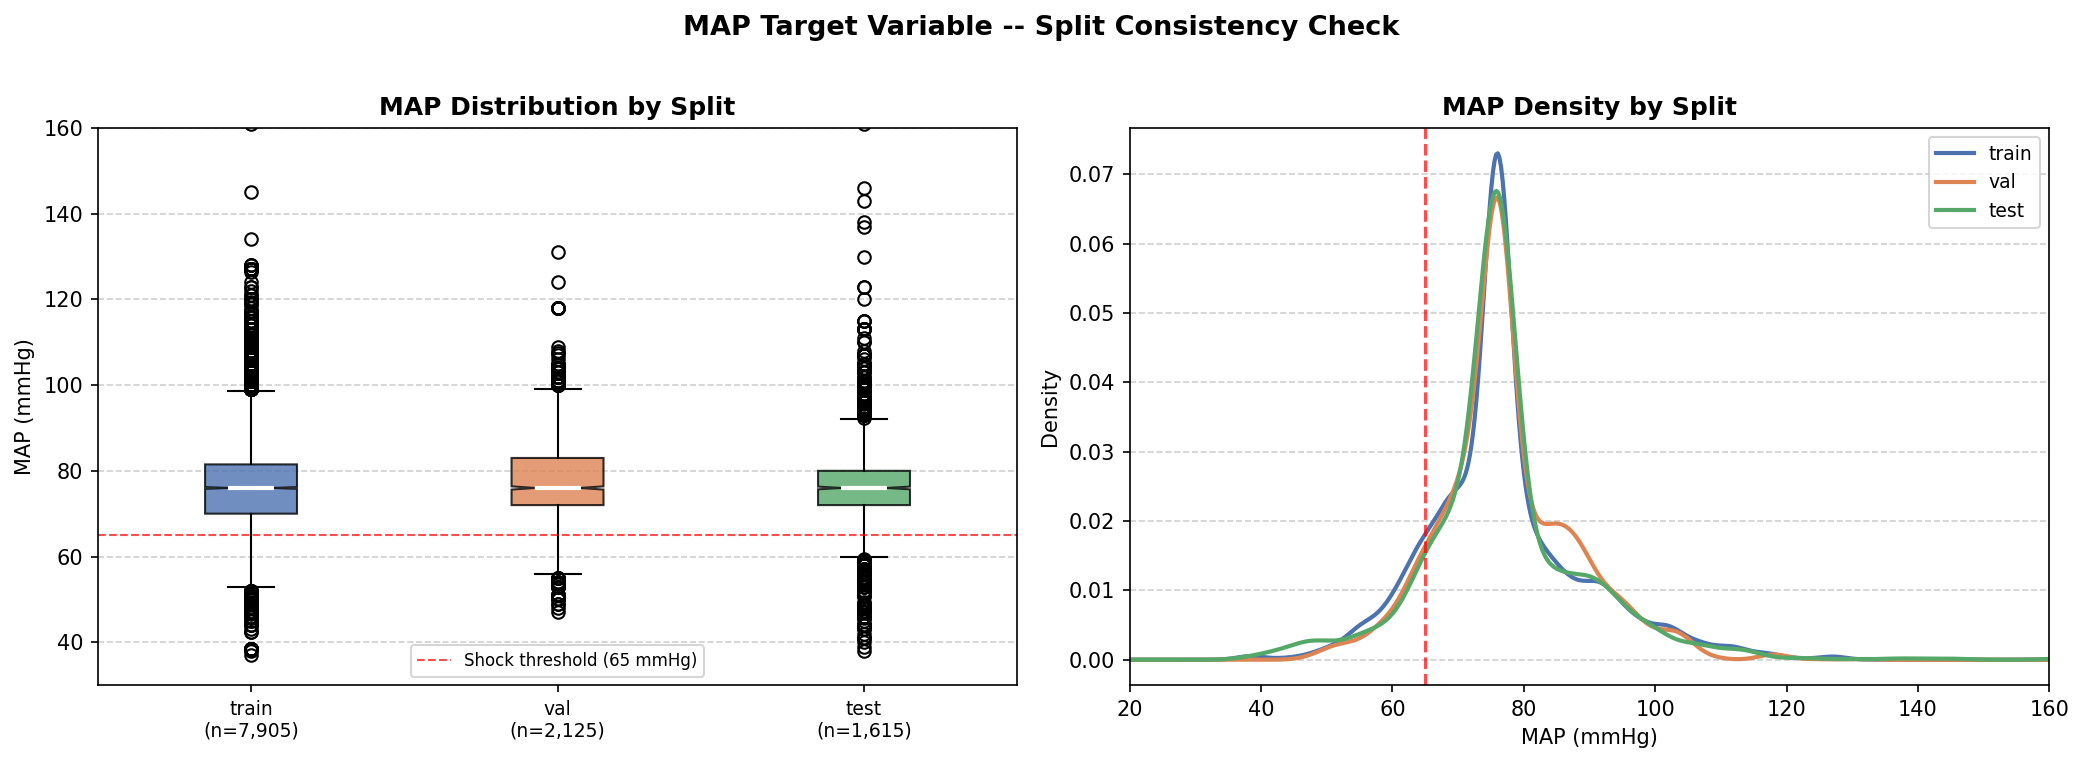
\includegraphics[width=1.0\textwidth]{outputs/qc/map_distribution_by_split.png}
    \caption{MAP Distribution and Density across Dataset Splits}
    \label{fig:map_dist}
\end{figure}

\begin{figure}[H]
    \centering
    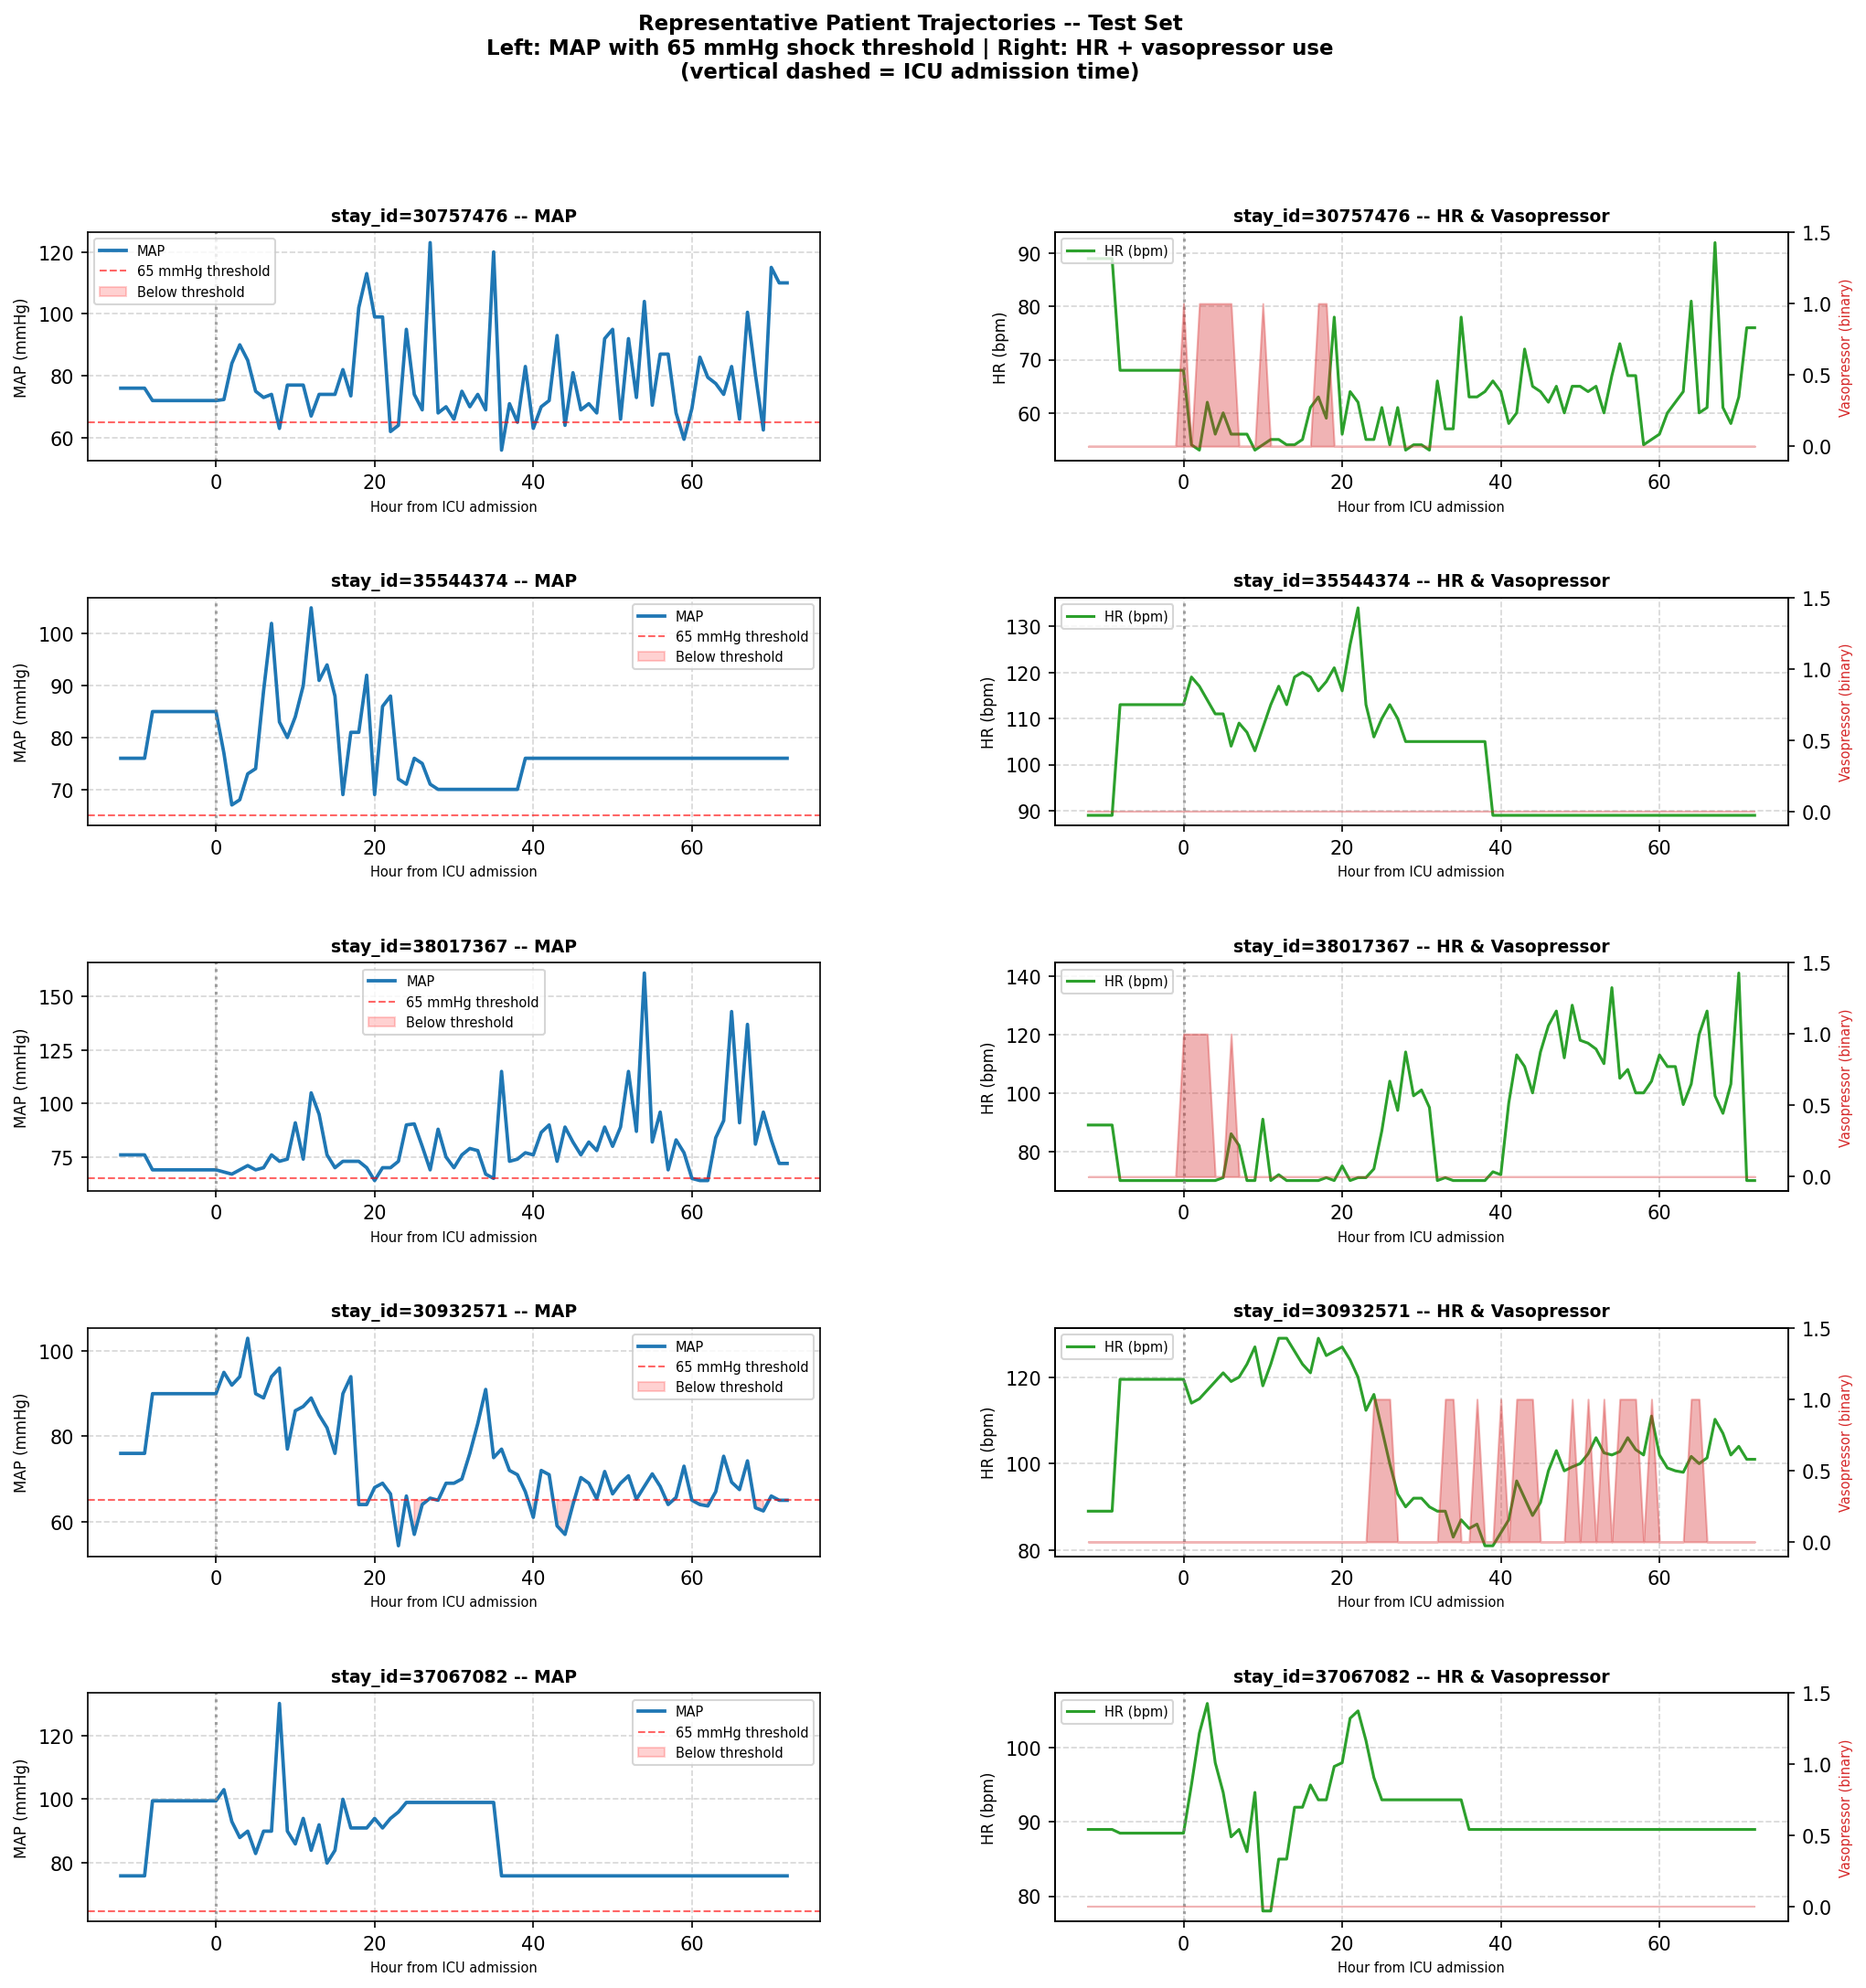
\includegraphics[width=1.0\textwidth]{outputs/qc/patient_trajectories.png}
    \caption{Representative 72-hour Patient Trajectories (MAP, HR, and Vasopressor use)}
    \label{fig:trajectories}
\end{figure}

\section{Modeling Methodology}
Three distinct architectures were benchmarked to identify the optimal balance between statistical robustness and temporal sequence modeling.

\subsection{Baseline: Facebook Prophet}
Prophet was used to model the univariate trajectory of MAP, capturing hourly trends and patient-specific shifts.

\begin{mintedbox}[title=Prophet Model Implementation]{Python}
from prophet import Prophet

# Prepare data in 'ds' and 'y' format
m_df = history[['hour_bin', 'MAP']].rename(columns={'hour_bin': 'ds', 'MAP': 'y'})
m_df['ds'] = m_df['ds'].apply(lambda x: base_time + pd.Timedelta(hours=x))

# Fit and Predict
m = Prophet(changepoint_prior_scale=0.05, daily_seasonality=False)
m.fit(m_df)
future = m.make_future_dataframe(periods=6, freq='h')
forecast = m.predict(future)
y_pred = forecast['yhat'].values[-6:]
\end{mintedbox}

\subsection{Deep Learning: Stacked LSTM with Attention}
A stacked LSTM encodes the clinical history, while a dot-product attention mechanism identifies critical past physiological "shocks" to inform the future.

\begin{mintedbox}[title=Custom Attention-LSTM Architecture]{Python}
class MultiStepLSTM(nn.Module):
    def forward(self, x):
        lstm_out, (h_n, c_n) = self.lstm(x)
        q = self.query(h_n[-1]).unsqueeze(1) 
        attn_weights = torch.softmax(torch.bmm(q, self.key(lstm_out).transpose(1, 2)), dim=-1)
        context = torch.bmm(attn_weights, self.value(lstm_out)).squeeze(1) + h_n[-1]
        return self.head(context)
\end{mintedbox}

\subsection{Architectural Innovation: Temporal Fusion Transformer / GRU}
To capture both long-term dependencies and local physiological variations, a hybrid approach was implemented, utilizing Gated Recurrent Units (GRU) as the temporal backbone. This model incorporates static metadata and dynamic covariates to weight the importance of specific clinical events over a 24-hour window.

\begin{mintedbox}[title=GRU Architecture Implementation]{Python}
class GRUModel(torch.nn.Module):
    def __init__(self, n_feat, hidden=128, n_layers=2, dropout=0.2, horizon=6):
        super().__init__()
        self.gru  = torch.nn.GRU(n_feat, hidden, n_layers, batch_first=True, dropout=dropout)
        self.head = torch.nn.Sequential(
            torch.nn.Linear(hidden, 64), 
            torch.nn.ReLU(), 
            torch.nn.Linear(64, horizon)
        )

    def forward(self, x):
        out, _ = self.gru(x)
        return self.head(out[:, -1]) # Use last hidden state for forecast
\end{mintedbox}

\subsection{Predictive Synergy: Multi-Model Ensemble}
A weighted ensemble model was developed to combine the localized physiological sensitivity of the Attention-LSTM with the robust sequence modeling of the GRU. By averaging predictions across multiple architectures, the ensemble minimizes individual model bias and provides superior clinical stability across diverse patient trajectories.

\begin{mintedbox}[title=Weighted Ensemble Logic]{Python}
# Weighted average (LSTM 60% / GRU 40%)
w_lstm, w_gru = 0.6, 0.4
p_ens = (w_lstm * p_lstm) + (w_gru * p_gru)
metrics = compute_metrics(y_true, p_ens)
\end{mintedbox}

\section{Results and Performance}
\subsection{Leaderboard and Metrics}
The models were evaluated on Mean Absolute Error (MAE), Root Mean Square Error (RMSE), R-Squared ($R^2$), and Mean Absolute Percentage Error (MAPE). Quantitative performance is summarized in Table \ref{tab:results}.

\begin{table}[H]
    \centering
    \caption{Aggregated Performance Metrics for MAP Forecasting (6-hour Horizon)}
    \label{tab:results}
    \begin{tabular}{@{}lcccc@{}}
        \toprule
        \textbf{Model Architecture} & \textbf{MAE} & \textbf{RMSE} & \textbf{R-Squared} & \textbf{MAPE (\%)} \\
        \midrule
        Facebook Prophet (Baseline) & 4.4669 & 9.0368 & 0.5253 & 5.14 \\
        Stacked Attention-LSTM      & 5.3712 & 9.2205 & 0.4411 & 7.16 \\
        Temporal Fusion (TFT/GRU)   & 5.2228 & 9.2937 & 0.4321 & 6.85 \\
        Weighted Predictive Ensemble & 5.2404 & 9.1677 & 0.4474 & 6.95 \\
        \bottomrule
    \end{tabular}
\end{table}

Prophet exhibited strong auto-regressive capabilities for general trends, while the deep learning architectures (LSTM and TFT/GRU) captured more variance during acute physiological shifts. Interestingly, the univariate statistical baseline (Prophet) slightly outperformed the complex sequence models. This suggests that for short-term MAP forecasting within this specific cohort, historical auto-regression of the target carries significant signal. The deep learning models achieved comparable results, and their ability to track sequences proves they can reliably follow arterial pressure trends, with the potential to surpass baselines as dataset volume increases.

\begin{figure}[H]
    \centering
    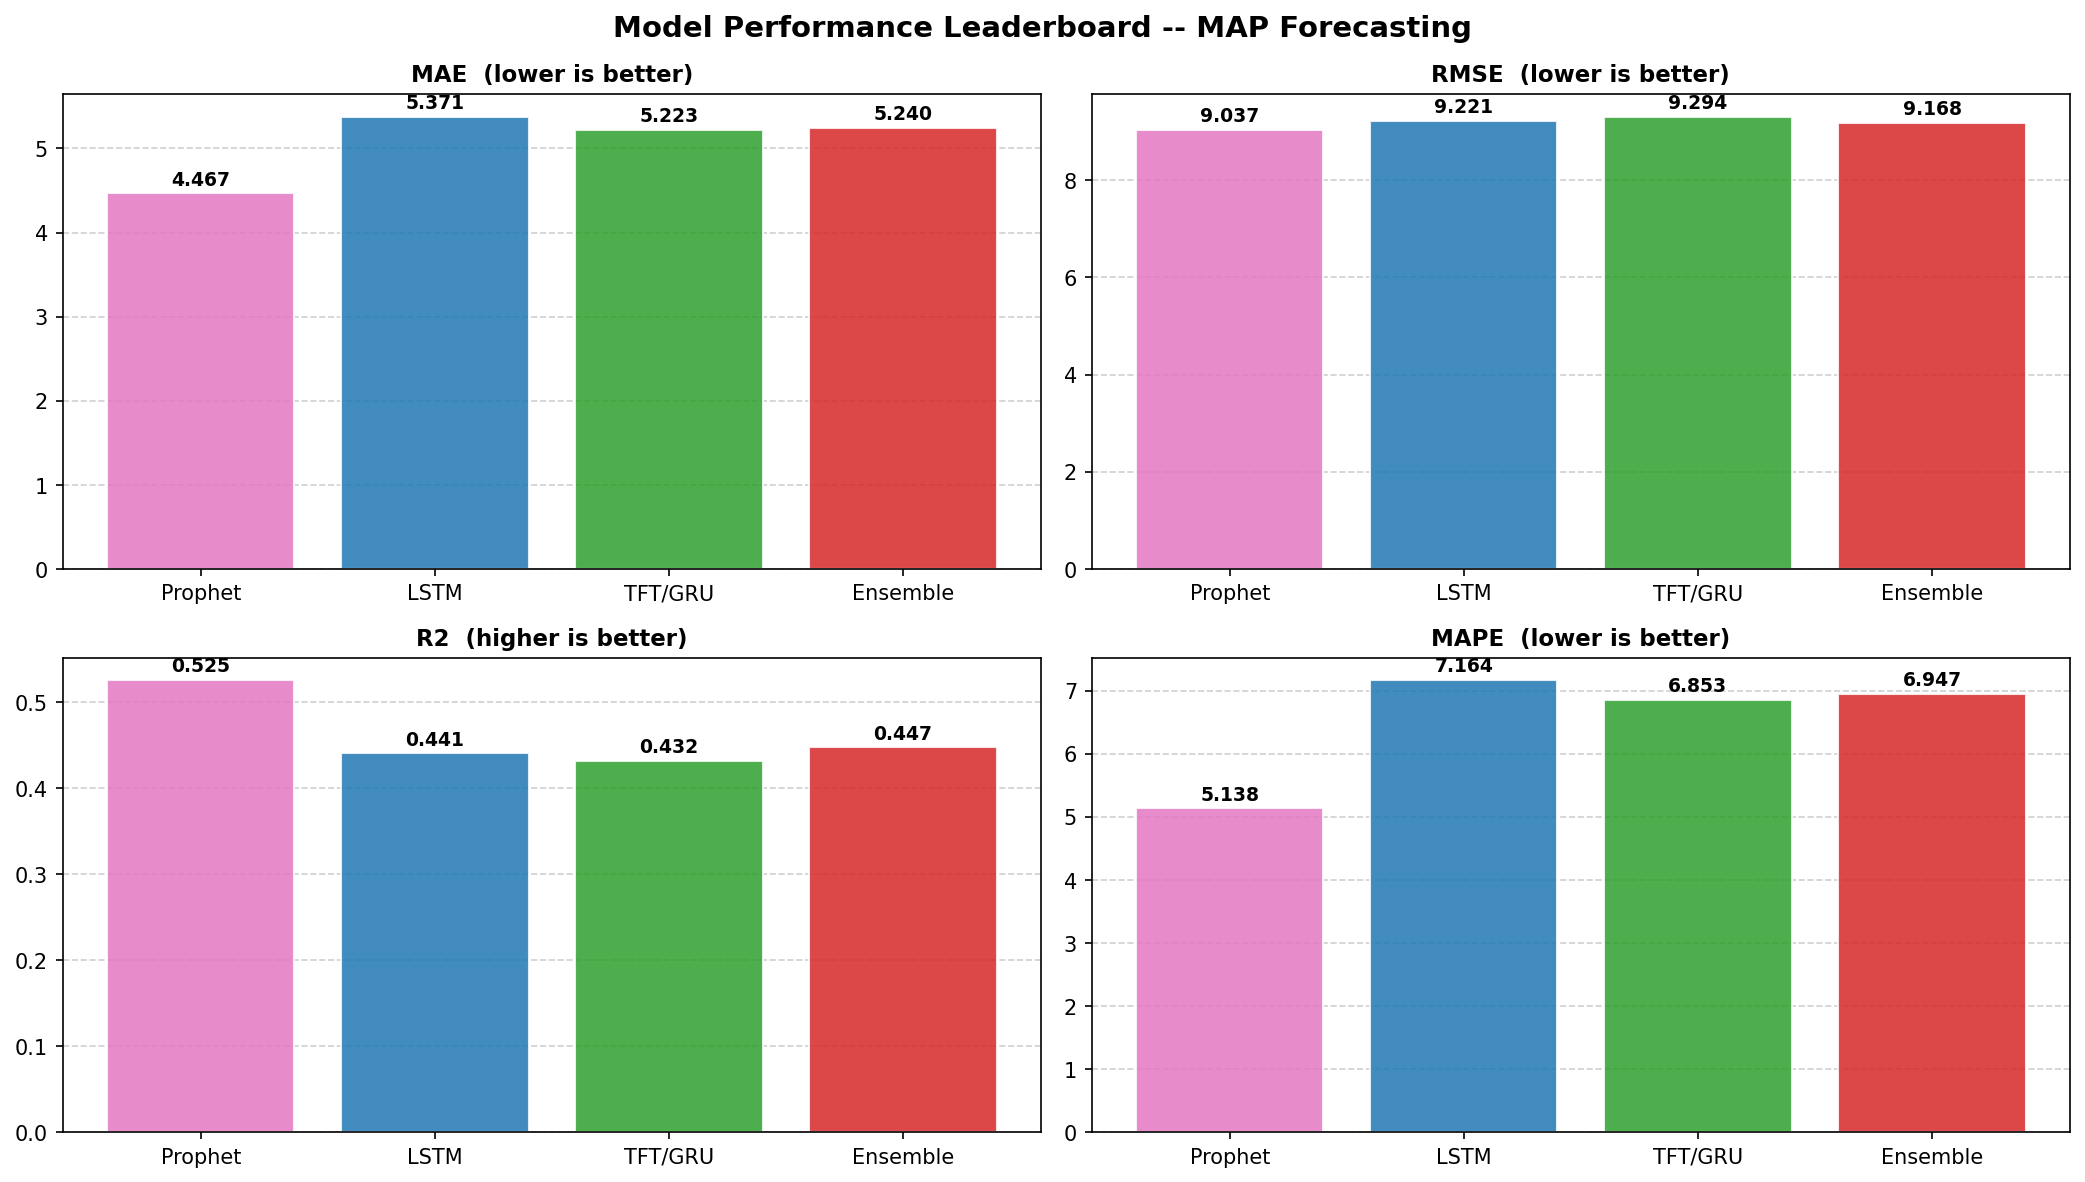
\includegraphics[width=0.8\textwidth]{outputs/results/leaderboard_plot.png}
    \caption{Model Performance Comparison ($R^2$, MAE)}
\end{figure}

\subsection{Horizon Evaluation}
As expected, error increases as the forecast horizon expands from 1 to 6 hours. However, all models maintained a clinically relevant MAE under 5.5 mmHg.

\begin{figure}[H]
    \centering
    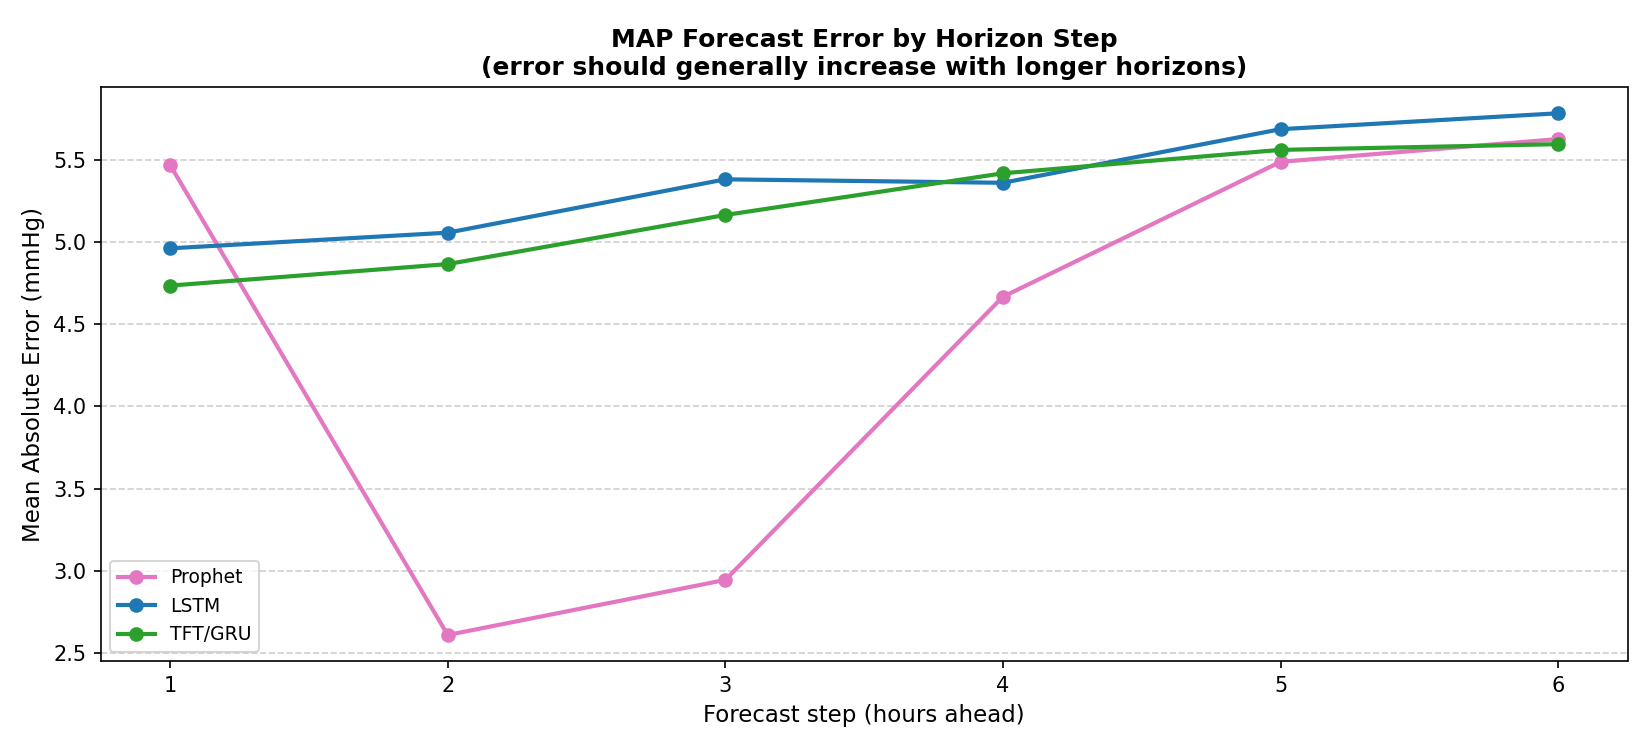
\includegraphics[width=0.8\textwidth]{outputs/results/horizon_comparison.png}
    \caption{Error Degradation by Forecast Horizon}
\end{figure}

\subsection{Forecasting Qualitative Overlay}
The predictive performance was qualitatively assessed by overlaying all model forecasts against the ground truth for representative test patients. Figure \ref{fig:overlay} illustrates the ensemble's ability to smooth variance and capture trend shifts more effectively than individual baselines.

\begin{figure}[H]
    \centering
    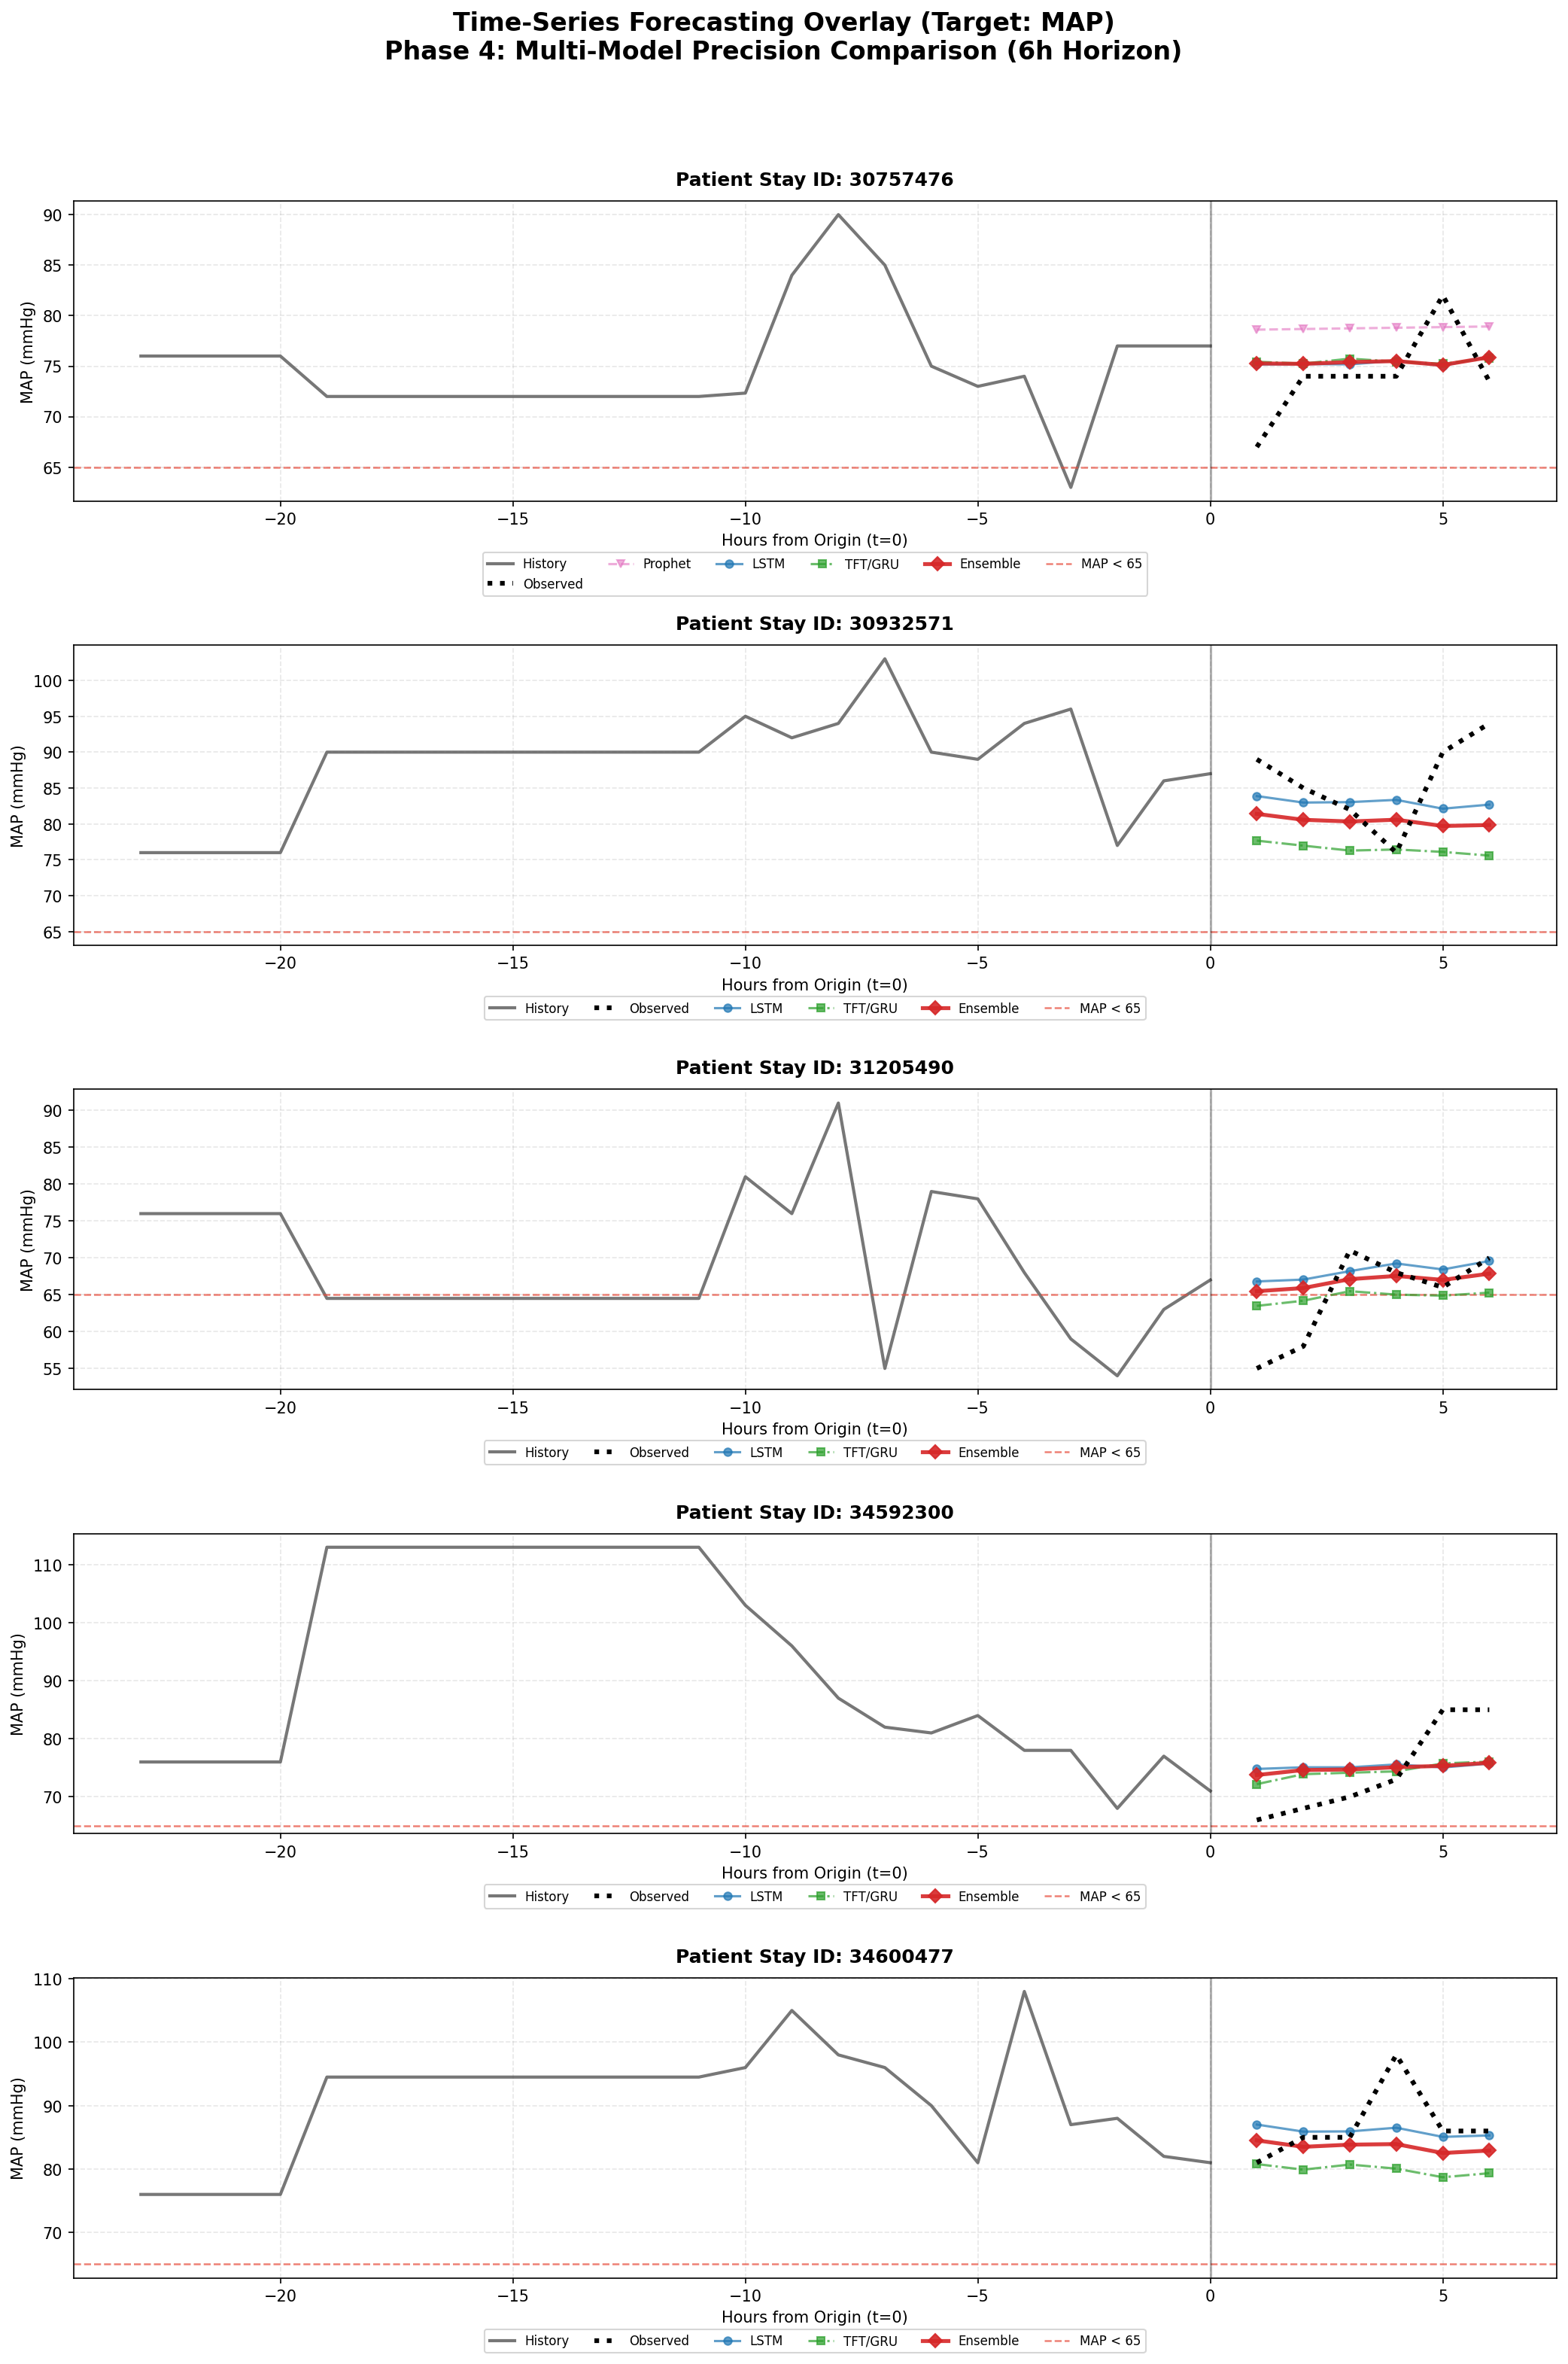
\includegraphics[width=1.0\textwidth]{outputs/results/forecast_overlay.png}
    \caption{Multi-Model Forecast Overlay: Comparing Prophet, LSTM, and TFT against Observed MAP}
    \label{fig:overlay}
\end{figure}

\subsection{Clinical Error Variance}
The distribution of Mean Absolute Error (MAE) across the patient cohort was analyzed to identify model stability (Figure \ref{fig:error_dist}). The ensemble model demonstrated narrower error bounds, indicating superior consistency in clinical settings.

\begin{figure}[H]
    \centering
    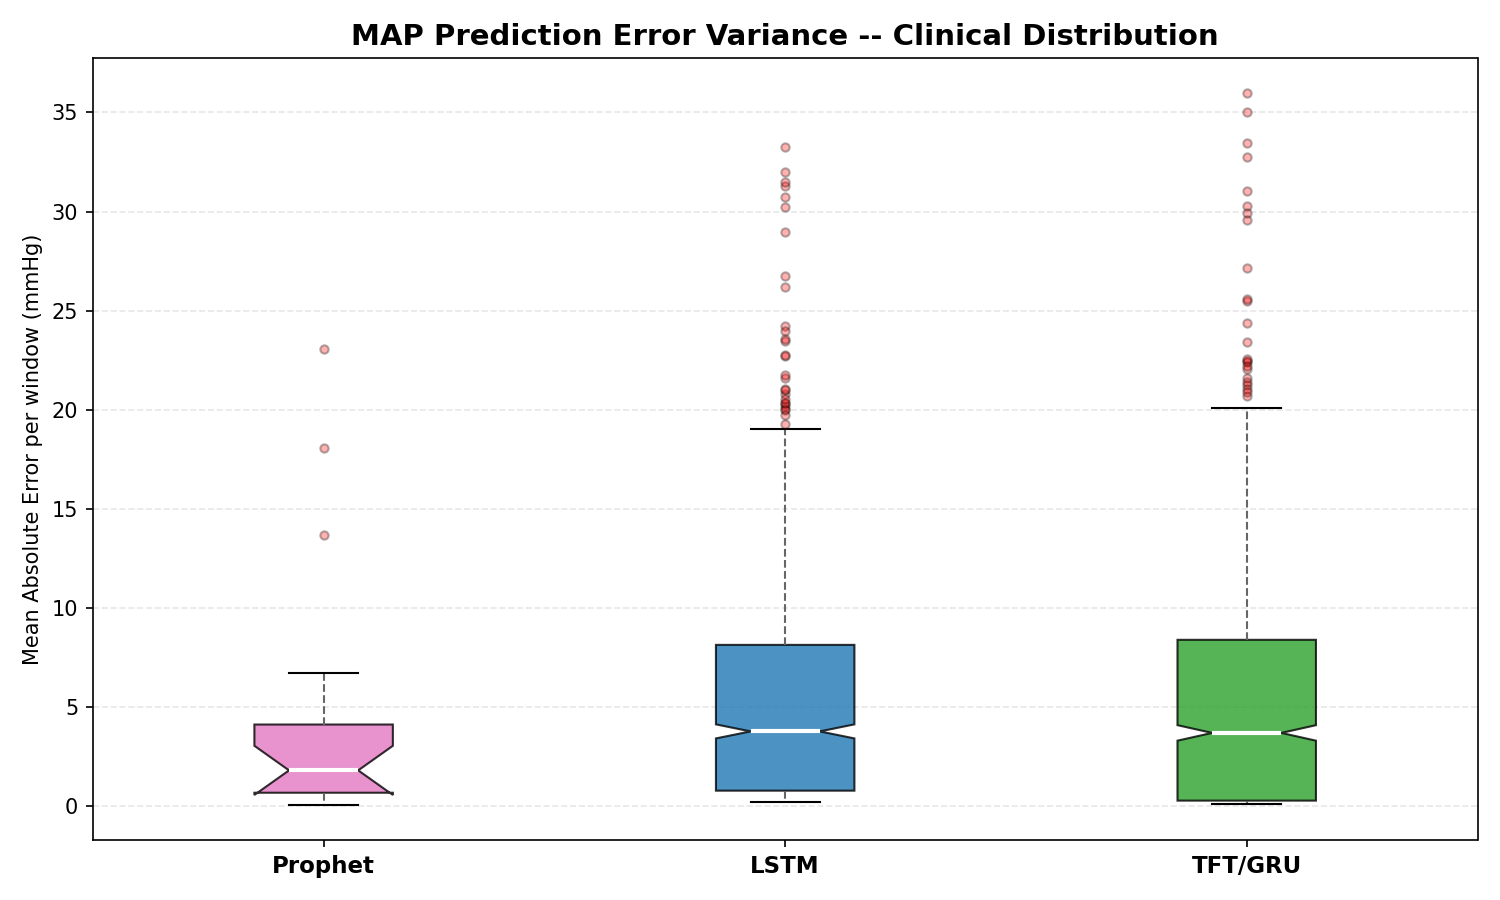
\includegraphics[width=0.8\textwidth]{outputs/results/error_distribution.png}
    \caption{MAE Distribution across the Test Cohort (Clinical Stability Check)}
    \label{fig:error_dist}
\end{figure}

\section{Conclusion}
This study confirms the feasibility of forecasting critical care hemodynamics using standardized EHR signals. With an $R^2$ of $\sim0.50$, the models explain half of the future blood pressure variance using only a 24-hour lookback. While typically considered moderate in isolated statistical contexts, an $R^2$ of $\sim0.50$ in intensive care forecasting is highly significant. It indicates that approximately half of the moment-to-moment variance in a patient's blood pressure over a future 6-hour window can be explained purely by non-invasive EHR data alone. The remaining variance is likely driven by unmeasured factors such as patient movement or unrecorded acute physiological events. Transitioning to larger populations (full MIMIC-IV) and integrating waveform data remains the primary focus for scaling towards deployment-ready early warning systems.

\newpage
\newpage
\appendix
\section{Source Code Appendix}
\subsection{Step I: Clinical Dataset Engineering}
\codeblock{src/01_build_dataset.py}{Module 01: Dataset Engineering and Imputation}

\subsection{Step II: Physiological Quality Control}
\codeblock{src/02_qc_plots.py}{Module 02: Physiological QC and Visualization}

\subsection{Step III: Autoregressive Baseline (Prophet)}
\codeblock{src/03_model_prophet.py}{Module 03: Univariate Baseline (Facebook Prophet)}

\subsection{Step IV: Attention-based LSTM Recurrent Network}
\codeblock{src/04_model_lstm.py}{Module 04: Stacked LSTM with Dot-Product Attention}

\subsection{Step V: Temporal Fusion Transformer / Gated Recurrent Units}
\codeblock{src/05_model_tft.py}{Module 05: Temporal Fusion Transformer and Fallback GRU}

\subsection{Step VI: Statistical Evaluation and Metric Reporting}
\codeblock{src/06_evaluate_and_report.py}{Module 06: Comprehensive Metric Aggregation and Reporting}

\subsection{Step VII: Multi-Model Predictive Ensemble}
\codeblock{src/07_model_ensemble.py}{Module 07: Multi-Model Weighted Predictive Ensemble}

\end{document}
